\chapter[Namelist options]{\hyperref[chap:namelist_sections]{Namelist options}}
\label{chap:namelist_tables}
Embedded links point to more detailed namelist information in the appendix.
\section[time\_management]{\hyperref[sec:nm_sec_time_management]{time\_management}}
\label{sec:nm_tab_time_management}
General time management is handled by the time\_management namelist record.
Included options handle time-related parts of MPAS, such as the calendar and if the simulation is a restart or not.

Users should use this record to specify the beginning time of the simulation,
and either the duration or the end of the simulation. Only the end or the
duration need to be specified as the other is derived within MPAS from the
beginning time and other specified one.

{\bf TBA: If both duration and stop are specified, then what happens?)}

\vspace{0.5in}
{\small
\begin{center}
\begin{longtable}{| p{2.0in} || p{4.0in} |}
	\hline
	{\bf Name} & {\bf Description} \endfirsthead
	\hline 
	{\bf Name} & {\bf Description} (Continued) \endhead
	\hline
	\hline
	\hyperref[subsec:nm_sec_config_do_restart]{config\_do\_restart} & Determines if the initial conditions should be read from a restart file, or an input file. \\
	\hline
	\hyperref[subsec:nm_sec_config_start_time]{config\_start\_time} & Timestamp describing the initial time of the simulation. If it is set to 'file', the initial time is read from restart\_timestamp. \\
	\hline
	\hyperref[subsec:nm_sec_config_stop_time]{config\_stop\_time} & Timestamp descriping the final time of the simulation. If it is set to 'none' the final time is determined from config\_start\_time and config\_run\_duration. \\
	\hline
	\hyperref[subsec:nm_sec_config_run_duration]{config\_run\_duration} & Timestamp describing the length of the simulation. If it is set to 'none' the duration is determined from config\_start\_time and config\_stop\_time. config\_run\_duration overrides inconsistent values of config\_stop\_time. \\
	\hline
	\hyperref[subsec:nm_sec_config_calendar_type]{config\_calendar\_type} & Selection of the type of calendar that should be used in the simulation. \\
	\hline
\end{longtable}
\end{center}
}
\section[io]{\hyperref[sec:nm_sec_io]{io}}
\label{sec:nm_tab_io}
The io namelist record provides options for modifications to the I/O system of
MPAS. These include frequency, file name, and parallelization options.

\vspace{0.5in}
{\small
\begin{center}
\begin{longtable}{| p{2.0in} || p{4.0in} |}
	\hline
	{\bf Name} & {\bf Description} \endfirsthead
	\hline 
	{\bf Name} & {\bf Description} (Continued) \endhead
	\hline
	\hline
	\hyperref[subsec:nm_sec_config_input_name]{config\_input\_name} & The path to the input file for the simulation. \\
	\hline
	\hyperref[subsec:nm_sec_config_output_name]{config\_output\_name} & The template path and name to the output file from the simulation. A time stamp is prepended to the extension of the file (.nc). \\
	\hline
	\hyperref[subsec:nm_sec_config_restart_name]{config\_restart\_name} & The template path and name to the restart file for the simulation. A time stamp is prepended to the extension of the file (.nc) both for input and output. \\
	\hline
	\hyperref[subsec:nm_sec_config_restart_timestamp_name]{config\_restart\_timestamp\_name} & The name of the file timestamps for latest restart files are written to. This file is also read when config\_start\_time is set to 'file' and config\_do\_restart is set to .true. \\
	\hline
	\hyperref[subsec:nm_sec_config_restart_interval]{config\_restart\_interval} & Timestamp determining how often a restart file should be written. \\
	\hline
	\hyperref[subsec:nm_sec_config_output_interval]{config\_output\_interval} & Timestamp determining how often an output file should be written. \\
	\hline
	\hyperref[subsec:nm_sec_config_stats_interval]{config\_stats\_interval} & Timestamp determining how often a global statistics files should be written. \\
	\hline
	\hyperref[subsec:nm_sec_config_write_stats_on_startup]{config\_write\_stats\_on\_startup} & Logical flag determining if statistics files should be written prior to the first time step. \\
	\hline
	\hyperref[subsec:nm_sec_config_write_output_on_startup]{config\_write\_output\_on\_startu-}\hyperref[subsec:nm_sec_config_write_output_on_startup]{p}& Logical flag determining if an output file should be written prior to the first time step. \\
	\hline
	\hyperref[subsec:nm_sec_config_frames_per_outfile]{config\_frames\_per\_outfile} & Integer specifying how many time frames should be included in an output file. Once the maximum is reached, a new output file is created. \\
	\hline
	\hyperref[subsec:nm_sec_config_pio_num_iotasks]{config\_pio\_num\_iotasks} & Integer specifying how many IO tasks should be used within the PIO library. A value of 0 causes all MPI tasks to also be IO tasks. IO tasks are requried to write contiguous blocks of data to a file. \\
	\hline
	\hyperref[subsec:nm_sec_config_pio_stride]{config\_pio\_stride} & Integer specifying the stride of each IO task. \\
	\hline
\end{longtable}
\end{center}
}
\section[time\_integration]{\hyperref[sec:nm_sec_time_integration]{time\_integration}}
\label{sec:nm_tab_time_integration}
The time integration namelist controls parameters that pertain to all time-stepping methods.  At present, Forward Euler is the only time integration method implemented.

\vspace{0.5in}
{\small
\begin{center}
\begin{longtable}{| p{2.0in} || p{4.0in} |}
	\hline
	{\bf Name} & {\bf Description} \endfirsthead
	\hline 
	{\bf Name} & {\bf Description} (Continued) \endhead
	\hline
	\hline
	\hyperref[subsec:nm_sec_config_dt]{config\_dt} & Length of model time-step. \\
	\hline
	\hyperref[subsec:nm_sec_config_time_integrator]{config\_time\_integrator} & Time integration method. \\
	\hline
\end{longtable}
\end{center}
}
\section[ALE\_vertical\_grid]{\hyperref[sec:nm_sec_ALE_vertical_grid]{ALE\_vertical\_grid}}
\label{sec:nm_tab_ALE_vertical_grid}
The MPAS-Ocean vertical grid is structured arbitrary Lagrangian-Eulerian (ALE).   ALE provides a great deal of freedom in the choice of vertical coordinate: when fully Eulerian, MPAS-Ocean is a z-level model with fixed thicknesses; when fully Lagrangian, there is no vertical transport between layers, and layers expand and contract like an isopycnal ocean model.  In between are many additional options, such as z-star where layers expand in proportion to the sea surface height, and sigma, where coordinates are terrain-following.

MPAS-Ocean employs the continuity equation,
\begin{eqnarray}
\label{ocean:continuity thickness}
\frac{\partial h_{k}}{\partial t} + D_k + w^t_k - w^t_{k+1} =0
\end{eqnarray}
for the ALE formulation, where variables are defined in Table \ref{oceanTable:ALE_variables}.  The ALE algorithm is as follows:
\begin{enumerate}
\item ALE step: Compute desired thickness for the new time,
\begin{eqnarray}
\label{ocean:desired thickness}
h_k^{ALE} = h_k^{rest} + h_k^{SSH} + h_k^{hf} + h_k^{min}
\end{eqnarray}
\item ALE step: Solve for vertical transport $w^t$ from (\ref{ocean:continuity thickness}),
\begin{eqnarray}
\label{ocean:vert tranport}
w^t_k = w^t_{k+1} - D_k - \frac{h^{ALE}_k - h^n_k}{\Delta t}
\end{eqnarray}
\item Solve for new thickness, $h_{k}^{n+1}$, using the continuity equation (\ref{ocean:continuity thickness}) within the time integration routine.
\end{enumerate}
The redundancy in steps 2 and 3 are intentional, so that step 2 is isolated within the ALE subroutine, and step 3 is solved in the timestepping subroutine in the identical manner as the tracer equation (\ref{ocean:tracer}).

The desired ALE thickness includes contributions from four terms (\ref{ocean:desired thickness}):
\begin{enumerate}
\item {\bf Resting thickness}, $h^{rest}$, is the layer thickness when the ocean is at rest, i.e. without SSH or internal perturbations.  For z-type coordinates, the resting thickness is constant in each horizontal layer.
\item {\bf SSH alteration}, $h^{SSH}$, alters layer thicknesses so that they change in proportion to the sea surface height (SSH),
\begin{eqnarray}
\label{ocean:h ssh}
   h_k^{SSH} =  \zeta \frac{W_k h^{rest}_k}{\sum_{k'=1}^{kmax}W_{k'}h^{rest}_{k'}}
\end{eqnarray}
The weights $W_k$ determine how SSH oscillations are distributed amongst the layers, as described in Table \ref{oceanTable:vertical coordinates}.
\item {\bf High-frequency thickness}, $h^{hf}$, allows high-frequency thickness oscillations, such as internal gravity waves, to be treated in a Lagrangian manner.  This is the ``z-tilde'' scheme of \citet{Leclair_Madec11om} described in the next section.
\item {\bf Minimum thickness alteration}, $h^{min}$, is the change in thickness required to enforce the minimum thickness in each cell.  When a cell is too thin, $h^{min}$ is positive, while nearby cells in the vertical incur a corresponding negative $h^{min}$ to conserve volume in the column.
\end{enumerate}
Of the four terms, resting thickness is always positive, while the others are small alterations about zero.  Summing a column,
\begin{eqnarray}
\sum_{k=1}^{kmax} h_k^{ALE} &=& \sum_{k=1}^{kmax} h_k^{rest} + \sum_{k=1}^{kmax}h_k^{SSH} + \sum_{k=1}^{kmax}h_k^{hf} + \sum_{k=1}^{kmax}h_k^{min} 
\nonumber \\
&=& H + \zeta + 0 + 0.
\nonumber
\end{eqnarray}
Thus the first two terms are always included so that the column thickness sums to $H+\zeta$, while the second two terms are optional and may be turned on with flags.

In order to assist users in choosing the correct settings, we provide a description of traditional vertical coordinate names in Table \ref{oceanTable:vertical coordinates}.
The vertical coordinate type also depends upon the set-up of the layerThickness variable in the initial condition file.  For all Z-type vertical coordinates, initial layer thicknesses are horizontally constant.  For sigma coordinates, layers are terrain-following and all layers are employed.  In this case, the user may still choose amongst the flags in SSH may be distributed through the column just like with z-type models in Table \ref{oceanTable:vertical coordinates}.

In order to run an isopycnal configuration, use config\_vert\_coord\_movement='impermeable\_interfaces' and set initial temperature and salinity to be constant within each layer.  All vertical tracer diffusion must be off so that the density in each layer remains constant.  For an isopycnal set-up, the equation of state is still called at each timestep, so a linear equation of state is recommended to avoid depth-dependancy of the density.  The user may choose a Montgomery Potential (\ref{ocean:Montgomery Potential}) or standard pressure gradient (\ref{ocean:grad p}); Montgomery Potential is a more common choice for isopycnal configurations, but both are tested and functional.  MPAS-Ocean does not support massless layers at this time, so isopycnal vertical coordinates may only be used for idealized domains.

\begin{table}[ht] 
\caption{Vertical coordinate settings for traditional names.}
\vspace{0.5cm} \centering 
\begin{tabular}{c c c c c c} 
\hline\hline flag name &  {\bf Z-Level} & {\bf Z-star} & {\bf weighted Z-star} &  {\bf isopycnal}  \\
\hline 
config\_vert\_ & 'fixed' & 'uniform\_stretching' & 'user\_specified' & 'impermeable\_ \\
coord\_movement & & & & interfaces'
\\
weights & $W_k =\left\{ \begin{array}{c} 1\; k=1\\ 0\; k>1 \end{array}\right.$ & $W_k=1\;\;\forall\;\;k$ & input file & not applicable \\
\hline 
\end{tabular} \label{oceanTable:vertical coordinates} 
\end{table}

\begin{table}[h!t] 
\caption{Variables used in ALE equation sets.  Column 3 shows the native horizontal grid location.  A subscript $k$ indicates indicates the layer index.  The $\nabla$ indicates a horizontal gradient within a single layer.} 
\vspace{0.5cm} \centering 
\begin{tabular}{c c c c } 
\hline\hline symbol &  name & grid &  notes  \\
\hline 
$D$  & thickness-weighted divergence & cell & $D_k = \nabla \cdot  \left( h_k {\bf u}_k \right)$  \\ 
${\bar D}$ & barotropic divergence & cell & ${\overline D} = \sum\limits_{k=1}^{kmax} D_k$  \\ 
$D'$  & baroclinic divergence & cell & $D'_k = D_k-\frac{h_k}{H}{\bar D}$  \\ 
$D^{lf}$  & low-frequency divergence & cell & see (\ref{ocean:Dlf})  \\ 
$D^{hf}$  & high-frequency divergence & cell & $D^{hf}_k = D'_k - D^{lf}_k$  \\ 
$h$  & layer thickness & cell &   \\ 
$h^{ALE}$  & desired ALE thickness & cell & see (\ref{ocean:desired thickness})  \\ 
$h^{rest}$  & resting thickness & cell &   \\ 
$h^{SSH}$  & SSH thickness alteration & cell & see (\ref{ocean:h ssh})  \\ 
$h^{hf}$  & high-freq. thickness alteration & cell &   see (\ref{ocean:hhf})  \\ 
$h^{min}$  & minimum thickness alteration & cell &   \\ 
$H$  & total resting thickness & cell & $H= \sum\limits_{k=1}^{kmax} h_k^{rest}$  \\ 
${\bf u}$  & velocity & edge &   \\ 
$w^t$ & vertical transport & cell  & top of layer in vertical \\
$W$  & SSH thickness weights & cell &   \\ 
$\tau_{Dlf}$  & frequency filter time scale & constant &   \\ 
$\tau_{hhf}$  & restoring time scale for $h^{hf}$ & constant &   \\ 
$\kappa_{hhf}$  & $h^{hf}$ diffusion & constant &   \\ 
$\zeta$  & sea surface height & cell &  $\zeta= \sum\limits_{k=1}^{kmax} h_k^{rest} - H$  \\ 
\hline 
\end{tabular} \label{oceanTable:ALE_variables} 
\end{table}


\vspace{0.5in}
{\small
\begin{center}
\begin{longtable}{| p{2.0in} || p{4.0in} |}
	\hline
	{\bf Name} & {\bf Description} \endfirsthead
	\hline 
	{\bf Name} & {\bf Description} (Continued) \endhead
	\hline
	\hline
	\hyperref[subsec:nm_sec_config_vert_coord_movement]{config\_vert\_coord\_movement} &  Determines the vertical coordinate movement type. 'uniform\_stretching' distributes SSH perturbations through all vertical levels (z-star vertical coordinate); 'fixed' places them all in the top level (z-level vertical coordinate); 'user\_specified' allows the input file to determine the distribution using the variable vertCoordMovementWeights (weighted z-star vertical coordinate); and 'impermeable\_interfaces' makes the vertical transport between layers zero, i.e.  $w^t=0$  (idealized isopycnal). \\
	\hline
	\hyperref[subsec:nm_sec_config_use_min_max_thickness]{config\_use\_min\_max\_thickness} & If true, a minimum and maximum thicknesses are enforced to prevent massless and very thick layers. \\
	\hline
	\hyperref[subsec:nm_sec_config_min_thickness]{config\_min\_thickness} & Minimum thickness allowed. \\
	\hline
	\hyperref[subsec:nm_sec_config_max_thickness_factor]{config\_max\_thickness\_factor} &  Maximum thickness allowed.  This is a factor times the resting thickness, i.e., maximum thickness = config\_max\_thickness\_factor* $h^{rest}$ . \\
	\hline
	\hyperref[subsec:nm_sec_config_set_restingThickness_to_IC]{config\_set\_restingThickness\_t-}\hyperref[subsec:nm_sec_config_set_restingThickness_to_IC]{o\_IC}& If true, set restingThickness to be the same as layerThickness upon start-up.  This only occurs when config\_do\_restart is false, i.e. on an initial run. \\
	\hline
	\hyperref[subsec:nm_sec_config_dzdk_positive]{config\_dzdk\_positive} & Determines if the positive Z axis is aligned with the positive K index direction. \\
	\hline
\end{longtable}
\end{center}
}
\section[ALE\_frequency\_filtered\_thickness]{\hyperref[sec:nm_sec_ALE_frequency_filtered_thickness]{ALE\_frequency\_filtered\_thickness}}
\label{sec:nm_tab_ALE_frequency_filtered_thickness}
The high-frequency thickness alteration, $h^{hf}$, in (\ref{ocean:\mode_desired thickness}) allows the thicknesses to oscillate so that high-frequency motions, such as internal gravity waves, are treated in a Lagrangian manner.  Low-freqency motions, such as seasonal changes or slow motions of water masses, are treated in an Eulerian manner.  This is the ``z-tilde'' scheme of \citet{Leclair_Madec11om}, which generally reduces spurious vertical mixing and preserves water mass properties.  Two additional prognostic equations are solved when config\_use\_freq\_filtered\_thickness is true,
\begin{eqnarray}
\label{ocean:\mode_Dlf}
 & \displaystyle
  \frac{\partial D^{lf}_k}{\partial t} = - \frac{2\pi}{\tau_{Dlf}} \left( D^{lf}_k - D'_k \right), 
\\ & \displaystyle
\label{ocean:\mode_hhf}
\frac{\partial h^{hf}_k}{\partial t} =  - D^{hf}_k - \frac{2\pi}{\tau_{hhf}} h^{hf}_k + \nabla_h\cdot \left( \kappa_{hhf} \nabla_h h^{hf}_k \right) 
\end{eqnarray}
where $\tau_{Dlf}$ is the filter timescale and other variables are defined in Table \ref{oceanTable:\mode_ALE_variables}.  This may be used in addition to any of the z-type or sigma-type vertical coordinates in Table \ref{oceanTable:\mode_vertical coordinates}.  Some combination of thickness restoring and diffusion are recommended to avoid long-term drift of $h^{hf}$ away from zero.




\vspace{0.5in}
{\small
\begin{center}
\begin{longtable}{| p{2.0in} || p{4.0in} |}
	\hline
	{\bf Name} & {\bf Description} \endfirsthead
	\hline 
	{\bf Name} & {\bf Description} (Continued) \endhead
	\hline
	\hline
	\hyperref[subsec:nm_sec_config_use_freq_filtered_thickness]{config\_use\_freq\_filtered\_thickn-}\hyperref[subsec:nm_sec_config_use_freq_filtered_thickness]{ess}&  If true,  $h^{hf}$  is included in the desired ALE thickness, and the prognostic equations for  $D^{lf}$  and  $h^{hf}$  are integrated in the code. \\
	\hline
	\hyperref[subsec:nm_sec_config_thickness_filter_timescale]{config\_thickness\_filter\_timescal-}\hyperref[subsec:nm_sec_config_thickness_filter_timescale]{e}&  Filter time scale for the low-frequency baroclinic divergence,  $\tau_{Dlf}$ . \\
	\hline
	\hyperref[subsec:nm_sec_config_use_highFreqThick_restore]{config\_use\_highFreqThick\_rest-}\hyperref[subsec:nm_sec_config_use_highFreqThick_restore]{ore}&  If true, the high frequency thickness prognostic equation ( $h^{hf}$ ) includes term 2 on the RHS, the restoring term.  The high frequency thickness is restored to zero with time scale  $\tau_{hhf}$ . \\
	\hline
	\hyperref[subsec:nm_sec_config_highFreqThick_restore_time]{config\_highFreqThick\_restore\_-}\hyperref[subsec:nm_sec_config_highFreqThick_restore_time]{time}&  Restoring time scale for high-frequency thickness,  $\tau_{hhf}$ . \\
	\hline
	\hyperref[subsec:nm_sec_config_use_highFreqThick_del2]{config\_use\_highFreqThick\_del2} &  If true, high frequency thickness prognostic equation ( $h^{hf}$ ) includes term 3 on the RHS, the diffusion term. \\
	\hline
	\hyperref[subsec:nm_sec_config_highFreqThick_del2]{config\_highFreqThick\_del2} &  Horizonal high frequency thickness diffusion,  $\kappa_{hhf}$ . \\
	\hline
\end{longtable}
\end{center}
}
\section[partial\_bottom\_cells]{\hyperref[sec:nm_sec_partial_bottom_cells]{partial\_bottom\_cells}}
\label{sec:nm_tab_partial_bottom_cells}
\documentclass[11pt]{report}

\usepackage{epsf,amsmath,amsfonts}
\usepackage{graphicx}

\setlength{\textwidth}{6.5in}
\setlength{\oddsidemargin}{0in}
\setlength{\evensidemargin}{0in}
\setlength{\textheight}{8.5in}
\setlength{\topmargin}{0in}

\begin{document}

\title{
Requirements and Design\\
Partial Bottom Cells}
\author{MPAS Development Team}

\maketitle
\tableofcontents

%-----------------------------------------------------------------------

\chapter{Summary}

Partial bottom cells (PBCs) allow bottom topography to be represented more realistically.  Currently, MPAS-Ocean only suports full ocean cells, so the bottom depth of a column is restricted to the depth of each vertical cell interface.  With partial bottom cells, the bottom depth may take on any value.  This is still a z-level-type formulation, where cells that are fully below the bottom depth are considered land cells.  The PBC formulation will work with z-level, z-star, and z-tilde formulations.

%figure template
%\begin{figure}
%  \center{\includegraphics[width=14cm]{./Figure1.pdf}}
%  \caption{A graphical representation of the discrete boundary.}
%  \label{Figure1}
%\end{figure} 

%-----------------------------------------------------------------------

\chapter{Requirements}

\section{Requirement: initial conditions with consistant variables}
Date last modified: 2012/10/15 \\
Contributors: Mark Petersen \\

The following variables must be consistent upon starting a new simulation with mpas-ocean: bottomDepth, maxLevelCell, thickness $h$, location of initial tracers in bottom cell.

\section{Requirement: horizontal advection}
Date last modified: 2012/08/01 \\
Contributors: Mark Petersen \\

Horizontal advection must take place through a thickness that accounts for the partial bottom cell at the bottom of the column.

\section{Requirement: pressure gradient}
Date last modified: 2012/08/01 \\
Contributors: Mark Petersen \\

Pressure gradients must not contain spurious effects due to the partial bottom cells.



%-----------------------------------------------------------------------

\chapter{Algorithmic Formulations}

\section{Design Solution: initial conditions with consistant variables}

Date last modified: 2012/10/15 \\
Contributors: Mark Petersen \\

The thickness variable {\tt h(k,iCell,iStep)} will continue to be the actual thickness of fluid in the cell.  
A new variable, {\tt bottomDepth(iCell)}, is the depth below the average sea surface height ($z=0$) in each cell, and is a positive number.    The variable {\tt maxLevelCell(iCell)} is an integer of the deepest active (water-filled) cell, and {\tt refBottomDepth(k)} is the depth of the bottom of each cell in z-level coordinates.  Note that depth variables are positive, $z$ variables are negative and decrease with greater depths, and the $k$ index increases with greater depth.

In generating the initial conditions (IC), the following steps are taken:
\begin{enumerate}
\item An additional parameter, {\tt max\_partial\_bottom\_cell}, may be set between zero and one, with default .95, in the initial condition generation.  Then {\tt bottomDepth} must be altered so that a partial bottom cell has a maximum of (say) 95\% land.  This parameter may be adjusted after testing. 
\item The thickness {\tt h} at {\tt k=maxLevelCell} is reduced to take into account the thickness removed by the partial bottom cell.
\item Initial tracer values in the bottom cell are interpolated to the center of the pbc, rather than the center of the full cell.
\item Check that {\tt bottomDepth} corresponds to {\tt maxLevelCell} (because they are redundant):\\
when {\tt k=maxLevelCell(iCell)}:\\
{\tt refBottomDepth(k)<bottomDepth(iCell)< refBottomDepth(k-1)}
\end{enumerate}

The ICs could be altered in basin.F or upon start-up with mpas.  We chose to alter the ICs in mpas to reduce the number and IC files and the complexity of IC generation.  The initial netcdf file (ocean.nc, produced by basin), include a realistic
 bottomDepth variable and thickness and tracer variables for full thickness cells.

Upon start-up with {\tt config\_do\_restart = .false.}, ICs are altered as described above.  An additional flag is used as follows:
\begin{itemize}
\item If running with pbcs, set {\tt config\_alter\_ICs\_for\_pbc='zlevel\_pbcs\_on'}. Then thin pbc cells
   will be changed, and thickness and tracers will be altered to match the pbcs (steps 1-3, above).
\item If running without pbcs, set {\tt config\_alter\_ICs\_for\_pbc='zlevel\_pbcs\_off'}. Then 
   bottomDepth will be altered so it is full cells everywhere.
   If your input file does not include bottomDepth, the false option will
   initialize bottomDepth correctly for a non-pbc run.
\item Set {\tt config\_alter\_ICs\_for\_pbc='no'} for isopycnal or sigma coordinates.
\end{itemize}

Consistency between {\tt bottomDepth} and {\tt maxLevelCell} is verified afterwards if {\tt config\_check\_zlevel\_consistency=.true.}


\section{Design Solution: horizontal advection}
Date last modified: 2012/08/01 \\
Contributors: Mark Petersen \\

{\bf Option 1: Do nothing (this option was chosen)}\\

If nothing is changed in the current code, {\tt h\_edge} is computed from from the thickness of nearby cells, regardless of PBCs in the bottom layer.  This is a clean and simple solution, but if PBCs are very thin, a cell could be evacuated of water.\\

{\bf Option 2: h\_edge is limited by minimum depth of neighboring cells}\\

In POP, the thickness of a U-cell is the minimum of the four surrounding T-Cells.  Likewise in MPAS-Ocean, one could compute the edge thickness using the minimum bottom depth of the two surrounding cells.  For the computation of {\tt h\_edge} using higher order advection methods, this will require further thought.

\section{Design Solution: pressure gradient}
Date last modified: 2012/08/01 \\
Contributors: Mark Petersen \\

{\bf Option 1: Do nothing (this option was chosen)}\\

MPAS-Ocean currently has two terms related to the pressure gradient,
\begin{equation}
- \frac{1}{\rho_0}\nabla p_k  - \frac{\rho g}{\rho_0}\nabla z^{mid}_k.
\end{equation}
where the gradient of $z^{mid}$ makes up pressure differences due to tilted levels.  However, in a stratified ocean, pressure gradient errors occur when the tilting of levels is large.  In a z-star system without PBCs, these perturbations are limited by the ratio of sea surface height to total depth, so only a few percent.  With the inclusion of PBCs, $z^{mid}$ could vary from one gridcell to the next by half the layer thickness.\\

{\bf Option 2: Interpolate T \& S to center of bottom cell for pressure computation}\\

If the pressure gradient errors are deemed to be too large, one could extrapolate the temperature and salinity values to the mid-depth of the bottom cell, and compute density and pressure at that location.  This will require a special case when {\tt k=maxLevelCell}.  There will need to be an extra case in the computation of $\nabla z^{mid}$ as well, so that $z^{mid}$ at the bottom cell is at the cell center.


%-----------------------------------------------------------------------

\chapter{Design and Implementation}

\section{Implementation: consistency between thickness and partial bottom cell variables}
Date last modified: 2012/08/01 \\
Contributors: Mark Petersen \\


\section{Implementation: horizontal advection}
Date last modified: 2012/08/01 \\
Contributors: Mark Petersen \\


\section{Implementation: pressure gradient}
Date last modified: 2012/08/01 \\
Contributors: Mark Petersen \\


%-----------------------------------------------------------------------

\chapter{Testing}

\section{Testing and Validation: Partial bottom cells}
Date last modified: 2012/08/01 \\
Contributors: Mark Petersen \\

Use the test problem, already in the repository, following Ilicak ea 2012 overflow test case (\#4).


%-----------------------------------------------------------------------

\end{document}

\vspace{0.5in}
{\small
\begin{center}
\begin{longtable}{| p{2.0in} || p{4.0in} |}
	\hline
	{\bf Name} & {\bf Description} \endfirsthead
	\hline 
	{\bf Name} & {\bf Description} (Continued) \endhead
	\hline
	\hline
	\hyperref[subsec:nm_sec_config_alter_ICs_for_pbcs]{config\_alter\_ICs\_for\_pbcs} & If true, initial conditions are altered according to the config\_pbc\_alteration\_type flag.  The alteration of layer thickness only occurs when config\_do\_restart is false, i.e. on an initial run. \\
	\hline
	\hyperref[subsec:nm_sec_config_pbc_alteration_type]{config\_pbc\_alteration\_type} & Determines the method of initial condition alteration for partial bottom cells.  'partial\_cell' alters layerThickness, interpolates all tracers in the bottom cell based on the bottomDepth variable, and alters bottomDepth to enforce the minimum pbc fraction.  'full\_cell' alters bottomDepth to have full cells everywhere, based on the refBottomDepth variable. \\
	\hline
	\hyperref[subsec:nm_sec_config_min_pbc_fraction]{config\_min\_pbc\_fraction} & Determines the minimum fraction of a cell altering the initial conditions can create.  The alteration of layer thickness only occurs when config\_do\_restart is false, i.e. on an initial run. \\
	\hline
	\hyperref[subsec:nm_sec_config_check_ssh_consistency]{config\_check\_ssh\_consistency} &  Enables a check to determine if the SSH is within 2m of the surface.  See equation for  $\zeta_i$ . \\
	\hline
\end{longtable}
\end{center}
}
\section[decomposition]{\hyperref[sec:nm_sec_decomposition]{decomposition}}
\label{sec:nm_tab_decomposition}
MPAS handles decomposing all variables into computational blocks. The
decomposition used needs to be specified at run time and is computed by an
external tool (e.g. metis). Additionally, MPAS supports multiple computational
blocks per MPI process, and the user may specify an additional decomposition
file which can specify the assignment of blocks to MPI processes. Run-time
parameters that control the run-time decomposition used are specified within
the decomposition namelist record.


\vspace{0.5in}
{\small
\begin{center}
\begin{longtable}{| p{2.0in} || p{4.0in} |}
	\hline
	{\bf Name} & {\bf Description} \endfirsthead
	\hline 
	{\bf Name} & {\bf Description} (Continued) \endhead
	\hline
	\hline
	\hyperref[subsec:nm_sec_config_num_halos]{config\_num\_halos} & Determines the number of halo cells extending from a blocks owned cells (Called the 0-Halo). The default of 3 is the minimum that can be used with monotonic advection. \\
	\hline
	\hyperref[subsec:nm_sec_config_block_decomp_file_prefix]{config\_block\_decomp\_file\_prefix} & Defines the prefix for the block decomposition file. Can include a path. The number of blocks is appended to the end of the prefix at run-time. \\
	\hline
	\hyperref[subsec:nm_sec_config_number_of_blocks]{config\_number\_of\_blocks} & Determines the number of blocks a simulation should be run with. If it is set to 0, the number of blocks is the same as the number of MPI tasks at run-time. \\
	\hline
	\hyperref[subsec:nm_sec_config_explicit_proc_decomp]{config\_explicit\_proc\_decomp} & Determines if an explicit processor decomposition should be used. This is only useful if multiple blocks per processor are used. \\
	\hline
	\hyperref[subsec:nm_sec_config_proc_decomp_file_prefix]{config\_proc\_decomp\_file\_prefix} & Defines the prefix for the processor decomposition file. This file is only read if config\_explicit\_proc\_decomp is .true. The number of processors is appended to the end of the prefix at run-time. \\
	\hline
\end{longtable}
\end{center}
}
\section[hmix]{\hyperref[sec:nm_sec_hmix]{hmix}}
\label{sec:nm_tab_hmix}
There are several choices of horizontal mixing schemes available for the 
momentum and tracer equations.  Each of these is a turbulence closure, 
and attempts to account for subgrid-scale mixing and diffusion.  These 
schemes have the practical effect of reducing grid-scale noise in the 
velocity and tracer fields, and improving numerical stability.

Each horizontal mixing scheme has its own namelist, and may be turned
on with the \verb|_use_| logical configuration flags.  Multiple
schemes may be run simultaneously.  The horizontal mixing terms in the
governing equations (\ref{ocean:momentum},
\ref{ocean:tracer}) are ${\bf D}^u_h$ for momentum and
$D^\varphi_h$ for tracers.  No horizontal mixing is applied to the
thickness equation.

All horizontal mixing coefficients can be set to scale with the mesh as $\rho_m^{-3/4}$ in equations (\ref{ocean:\mode_h_mom_del2}, \ref{ocean:\mode_h_tr_del2}, \ref{ocean:\mode_h_mom_del4}, \ref{ocean:\mode_h_tr_del4}).  The mesh density, $\rho_m$, is a variable in the input and restart file.  It can vary between zero and one, and is one in the highest resolution region.  Scaling with the mesh can be turned off, as described in the options below.

The anticipated potential Vorticity (APV) method is a parameterization of the effects of subgrid or unresolved scales on those explicitly resolved \citep{Vallis_Hua88jas}.  It contributes an upstream bias to the vorticity in the del2 and del4 momentum terms as follows,
\begin{equation}
\eta_{apv} = \eta - c_{apv} dt \left({\bf u}\cdot \nabla \eta\right),
\end{equation}
where the altered vorticity $\eta_{apv}$ is used in equations (\ref{ocean:\mode_h_mom_del2}, \ref{ocean:\mode_h_mom_del4a}, \ref{ocean:\mode_h_mom_del4b}).

\vspace{0.5in}
{\small
\begin{center}
\begin{longtable}{| p{2.0in} || p{4.0in} |}
	\hline
	{\bf Name} & {\bf Description} \endfirsthead
	\hline 
	{\bf Name} & {\bf Description} (Continued) \endhead
	\hline
	\hline
	\hyperref[subsec:nm_sec_config_hmix_scaleWithMesh]{config\_hmix\_scaleWithMesh} &  If false, del2 and del4 coefficients are constant throughout the mesh (equivalent to setting  $\rho_m=1$  throughout the mesh).  If true, these coefficients scale as mesh density to the -3/4 power. \\
	\hline
	\hyperref[subsec:nm_sec_config_maxMeshDensity]{config\_maxMeshDensity} & Global maximum of the mesh density \\
	\hline
	\hyperref[subsec:nm_sec_config_apvm_scale_factor]{config\_apvm\_scale\_factor} &  Anticipated potential vorticity (APV) method scale factor,  $c_{apv}$ .  When zero, APV is off. \\
	\hline
\end{longtable}
\end{center}
}
\section[hmix\_del2]{\hyperref[sec:nm_sec_hmix_del2]{hmix\_del2}}
\label{sec:nm_tab_hmix_del2}
The ``del2'', or Laplacian, turbulence closures are
\begin{eqnarray}
\label{ocean:\mode_h_mom_del2}
& {\bf D}^u_h=\displaystyle\frac{\nu_h}{\rho_m^{3/4}} \nabla^2 {\bf u} 
= \displaystyle\frac{\nu_h}{\rho_m^{3/4}}(\nabla \delta + {\bf 
k}\times \nabla \eta),\\
\label{ocean:\mode_h_tr_del2}
& D^\varphi_h = \nabla\cdot\left(h 
   \displaystyle\frac{\kappa_h}{\rho_m^{3/4}} \nabla\varphi \right)
\end{eqnarray}
for momentum and tracers, respectively.  Variable definitions appear in Tables \ref{oceanTable:variables} and \ref{oceanTable:variables_Greek}.  The momentum diffusion is in divergence-vorticity form because it is a natural discretization of the vector Laplacian operator with a C-grid staggering.  

The Laplacian operator smooths the momentum and 
tracer fields, and smooths more strongly at small scales than at large 
scales.  This operator is the two dimensional form of the heat equation, 
$u_t=\nu u_{xx}$, described in introductory books on partial 
differential equations.  The strength of mixing is controlled by the 
viscosity, $\nu_h$, for the momentum equation, and the diffusion, 
$\kappa_h$, for the tracer equation.

\vspace{0.5in}
{\small
\begin{center}
\begin{longtable}{| p{2.0in} || p{4.0in} |}
	\hline
	{\bf Name} & {\bf Description} \endfirsthead
	\hline 
	{\bf Name} & {\bf Description} (Continued) \endhead
	\hline
	\hline
	\hyperref[subsec:nm_sec_config_use_mom_del2]{config\_use\_mom\_del2} & If true, Laplacian horizontal mixing is used on the momentum equation. \\
	\hline
	\hyperref[subsec:nm_sec_config_use_tracer_del2]{config\_use\_tracer\_del2} & If true, Laplacian horizontal mixing is used on the tracer equation. \\
	\hline
	\hyperref[subsec:nm_sec_config_mom_del2]{config\_mom\_del2} &  Horizonal viscosity,  $\nu_h$ . \\
	\hline
	\hyperref[subsec:nm_sec_config_tracer_del2]{config\_tracer\_del2} &  Horizonal diffusion,  $\kappa_h$ . \\
	\hline
\end{longtable}
\end{center}
}
\section[hmix\_del4]{\hyperref[sec:nm_sec_hmix_del4]{hmix\_del4}}
\label{sec:nm_tab_hmix_del4}
The ``del4'', or biharmonic, turbulence closures are
\begin{eqnarray}
\label{ocean:\mode_h_mom_del4}
& {\bf D}^u_h=-\displaystyle\frac{\nu_h}{\rho_m^{3/4}} \nabla^4 {\bf u} \\
\label{ocean:\mode_h_tr_del4}
& D^\varphi_h = -\nabla\cdot\left(h \displaystyle\frac{\kappa_h}{\rho_m^{3/4}} \nabla \left[\nabla\cdot\left(h \nabla\varphi \right) \right] \right)
\end{eqnarray}
for momentum and tracers  These are both computed by applying the Laplacian operator twice.  For momentum, this can be written in terms of divergence and vorticity as
\begin{eqnarray}
&\delta=\nabla\cdot{\bf u}\\
&\eta={\bf k} \cdot \left( \nabla \times {\bf u} \right)+f\\
\label{ocean:\mode_h_mom_del4a}
&\nabla^2{\bf u}=(\nabla \delta + {\bf k}\times \nabla \eta) \\
&\delta_2=\nabla\cdot(\nabla^2{\bf u})\\
&\eta_2={\bf k} \cdot \left( \nabla \times (\nabla^2{\bf u}) \right)+f\\
\label{ocean:\mode_h_mom_del4b}
& {\bf D}^u_h= \displaystyle\frac{\nu_h}{\rho_m^{3/4}} (\nabla \delta_2 + {\bf k}\times \nabla \eta_2).
\end{eqnarray}
The biharmonic operator is similar to the Laplacian operator, but smooths more strongly at high wavenumbers.  

\vspace{0.5in}
{\small
\begin{center}
\begin{longtable}{| p{2.0in} || p{4.0in} |}
	\hline
	{\bf Name} & {\bf Description} \endfirsthead
	\hline 
	{\bf Name} & {\bf Description} (Continued) \endhead
	\hline
	\hline
	\hyperref[subsec:nm_sec_config_use_mom_del4]{config\_use\_mom\_del4} & If true, biharmonic horizontal mixing is used on the momentum equation. \\
	\hline
	\hyperref[subsec:nm_sec_config_use_tracer_del4]{config\_use\_tracer\_del4} & If true, biharmonic horizontal mixing is used on the tracer equation. \\
	\hline
	\hyperref[subsec:nm_sec_config_mom_del4]{config\_mom\_del4} & Coefficient for horizontal biharmonic operator on momentum. \\
	\hline
	\hyperref[subsec:nm_sec_config_tracer_del4]{config\_tracer\_del4} & Coefficient for horizontal biharmonic operator on tracers. \\
	\hline
\end{longtable}
\end{center}
}
\section[hmix\_Leith]{\hyperref[sec:nm_sec_hmix_Leith]{hmix\_Leith}}
\label{sec:nm_tab_hmix_Leith}
The \cite{Leith:1996wu} closure is the enstrophy-cascade analogy to the \cite{Smagorinsky:1963wc} energy-cascade closure, i.e.  the Leith closure assumes an inertial range of enstrophy flux moving toward the grid scale. The assumption of an enstrophy cascade and dimensional analysis produces right-hand-side dissipation, $\bf{D}^u_h$, of velocity of the form

\begin{equation}
\label{eq:\mode_Leith}
{\bf D}^u_h =\nabla \cdot \left( \nu_h \nabla {\bf u} \right) = \nabla \cdot \left( \Gamma \left| \nabla \omega  \right| \left( \Delta x \right)^3 \nabla \bf{u} \right)
\end{equation}
where $\omega$ is the relative vorticity, ${\bf u}$ is the horizontal velocity, $\Delta x$ is the local grid spacing and $\Gamma$ is a non-dimensional, $O(1)$ parameter. This beta release approximates the RHS of the \ref{eq:Leith} as

\begin{equation}
\bf{D}^u_h=\nu_\ast \nabla_h^2 {\bf u}
\end{equation}
where the $\nabla^2 {\bf u}$ is computed using the form shown in \ref{ocean:\mode_h_mom_del4a}. Future releases will remove this approximation by computing the rate-of-strain, i.e. $\nabla {\bf u}$, directly.

\vspace{0.5in}
{\small
\begin{center}
\begin{longtable}{| p{2.0in} || p{4.0in} |}
	\hline
	{\bf Name} & {\bf Description} \endfirsthead
	\hline 
	{\bf Name} & {\bf Description} (Continued) \endhead
	\hline
	\hline
	\hyperref[subsec:nm_sec_config_use_Leith_del2]{config\_use\_Leith\_del2} & If true, the Leith enstrophy-cascade closure is turned on \\
	\hline
	\hyperref[subsec:nm_sec_config_Leith_parameter]{config\_Leith\_parameter} & Non-dimensional Leith closure parameter \\
	\hline
	\hyperref[subsec:nm_sec_config_Leith_dx]{config\_Leith\_dx} & Characteristic length scale, usually the smallest dx in the mesh \\
	\hline
	\hyperref[subsec:nm_sec_config_Leith_visc2_max]{config\_Leith\_visc2\_max} & Upper bound on the allowable value of Leith-computed viscosity \\
	\hline
\end{longtable}
\end{center}
}
\section[standard\_GM]{\hyperref[sec:nm_sec_standard_GM]{standard\_GM}}
\label{sec:nm_tab_standard_GM}
The Gent-McWilliams eddy parameterization is currently a stub, and is not available in the current release.  Watch this space in a future release!

\vspace{0.5in}
{\small
\begin{center}
\begin{longtable}{| p{2.0in} || p{4.0in} |}
	\hline
	{\bf Name} & {\bf Description} \endfirsthead
	\hline 
	{\bf Name} & {\bf Description} (Continued) \endhead
	\hline
	\hline
	\hyperref[subsec:nm_sec_config_h_kappa]{config\_h\_kappa} & kappa parameter for Gent-McWilliams eddy parameterization \\
	\hline
	\hyperref[subsec:nm_sec_config_h_kappa_q]{config\_h\_kappa\_q} & kappa-q parameter for Gent-McWilliams eddy parameterization \\
	\hline
\end{longtable}
\end{center}
}
\section[hmix\_del2\_tensor]{\hyperref[sec:nm_sec_hmix_del2_tensor]{hmix\_del2\_tensor}}
\label{sec:nm_tab_hmix_del2_tensor}
A tensor version of the ``del2'' operator is provided for the momentum closure,
\begin{eqnarray}
\label{ocean:h_mom_del2_tensor}
& {\bf D}^u_h = \nabla\cdot\left( 
   \displaystyle\frac{\nu_h}{\rho_m^{3/4}} \nabla {\bf u}  \right).
\end{eqnarray}
The standard form for the del2 momentum closure is the divergence-vorticity form, described in the hmix\_del2 namelist above.  The tensor-based mixing operations are provided to show the functionality of the tensor subroutines.  Tensor-based del2 mixing is not fully vetted and not recommended for production simulations.

\vspace{0.5in}
{\small
\begin{center}
\begin{longtable}{| p{2.0in} || p{4.0in} |}
	\hline
	{\bf Name} & {\bf Description} \endfirsthead
	\hline 
	{\bf Name} & {\bf Description} (Continued) \endhead
	\hline
	\hline
	\hyperref[subsec:nm_sec_config_use_mom_del2_tensor]{config\_use\_mom\_del2\_tensor} & If true, tensor-based Laplacian horizontal mixing is used on the momentum equation.  The tensor-based mixing operations are provided to show the functionality of the tensor subroutines.  Tensor-based del2 mixing is not fully vetted and not recommended for production simulations. \\
	\hline
	\hyperref[subsec:nm_sec_config_mom_del2_tensor]{config\_mom\_del2\_tensor} &  Horizonal viscosity,  $\nu_h$ . \\
	\hline
\end{longtable}
\end{center}
}
\section[hmix\_del4\_tensor]{\hyperref[sec:nm_sec_hmix_del4_tensor]{hmix\_del4\_tensor}}
\label{sec:nm_tab_hmix_del4_tensor}
A tensor version of the ``del4'' operator is provided for the momentum closure,
\begin{eqnarray}
\label{ocean:\mode_h_mom_del4_tensor}
& {\bf D}^u_h = \nabla\cdot\left( 
   \displaystyle\frac{\nu_h}{\rho_m^{3/4}} \nabla 
\left[
\nabla\cdot \left(
   \displaystyle \nabla {\bf u} \right)  \right]
  \right).
\end{eqnarray}
The standard form for the del4 momentum closure is the divergence-vorticity form, described in the hmix\_del4 namelist above.  The tensor-based mixing operations are provided to show the functionality of the tensor subroutines.  Tensor-based del4 mixing is not fully vetted and not recommended for production simulations.

\vspace{0.5in}
{\small
\begin{center}
\begin{longtable}{| p{2.0in} || p{4.0in} |}
	\hline
	{\bf Name} & {\bf Description} \endfirsthead
	\hline 
	{\bf Name} & {\bf Description} (Continued) \endhead
	\hline
	\hline
	\hyperref[subsec:nm_sec_config_use_mom_del4_tensor]{config\_use\_mom\_del4\_tensor} & If true, tensor-based biharmonic horizontal mixing is used on the momentum equation.  The tensor-based mixing operations are provided to show the functionality of the tensor subroutines.  Tensor-based del4 mixing is not fully vetted and not recommended for production simulations. \\
	\hline
	\hyperref[subsec:nm_sec_config_mom_del4_tensor]{config\_mom\_del4\_tensor} & Coefficient for horizontal biharmonic operator on momentum. \\
	\hline
\end{longtable}
\end{center}
}
\section[Rayleigh\_damping]{\hyperref[sec:nm_sec_Rayleigh_damping]{Rayleigh\_damping}}
\label{sec:nm_tab_Rayleigh_damping}
A linear damping toward a state of rest is available with this namelist option.  It is implemented with a term on the RHS of the momentum equation (\ref{ocean:momentum}) of the form 
\begin{equation}
{\cal F}^u = -c_R {\bf u}.
\end{equation}


\vspace{0.5in}
{\small
\begin{center}
\begin{longtable}{| p{2.0in} || p{4.0in} |}
	\hline
	{\bf Name} & {\bf Description} \endfirsthead
	\hline 
	{\bf Name} & {\bf Description} (Continued) \endhead
	\hline
	\hline
	\hyperref[subsec:nm_sec_config_Rayleigh_friction]{config\_Rayleigh\_friction} & If true, Rayleigh friction is included in the momentum equation. \\
	\hline
	\hyperref[subsec:nm_sec_config_Rayleigh_damping_coeff]{config\_Rayleigh\_damping\_coeff} &  Inverse-time coefficient for the Rayleigh damping term,  $c_R$ . \\
	\hline
\end{longtable}
\end{center}
}
\section[vmix]{\hyperref[sec:nm_sec_vmix]{vmix}}
\label{sec:nm_tab_vmix}
\textbf{NOTE}: The functionality of this namelist has been superceded by the CVMix package, which has it's own namelist.  vmix is defunct and may be depracated in a future release.  Use of this parameterization is not recommended.

\vspace{0.5in}
{\small
\begin{center}
\begin{longtable}{| p{2.0in} || p{4.0in} |}
	\hline
	{\bf Name} & {\bf Description} \endfirsthead
	\hline 
	{\bf Name} & {\bf Description} (Continued) \endhead
	\hline
	\hline
	\hyperref[subsec:nm_sec_config_convective_visc]{config\_convective\_visc} & Value of vertical viscosity to be used in unstable conditions (i.e. Richardson number less than zero) \\
	\hline
	\hyperref[subsec:nm_sec_config_convective_diff]{config\_convective\_diff} & Value of vertical diffusion to be used in unstable conditions (i.e. Richardson number less than zero) \\
	\hline
\end{longtable}
\end{center}
}
\section[vmix\_const]{\hyperref[sec:nm_sec_vmix_const]{vmix\_const}}
\label{sec:nm_tab_vmix_const}
Here the vertical viscosity $\nu_v$ and diffusion $\kappa_v$ are simply constant throughout the domain.  This option is useful for testing and idealized domains but is not appropriate for real-world simulations, as the deep ocean should have much less mixing that the mixed layer.

\vspace{0.5in}
{\small
\begin{center}
\begin{longtable}{| p{2.0in} || p{4.0in} |}
	\hline
	{\bf Name} & {\bf Description} \endfirsthead
	\hline 
	{\bf Name} & {\bf Description} (Continued) \endhead
	\hline
	\hline
	\hyperref[subsec:nm_sec_config_use_const_visc]{config\_use\_const\_visc} & If true, constant vertical viscosity is included in the momentum equation \\
	\hline
	\hyperref[subsec:nm_sec_config_use_const_diff]{config\_use\_const\_diff} & If true, constant vertical diffusion is included in the tracer equation \\
	\hline
	\hyperref[subsec:nm_sec_config_vert_visc]{config\_vert\_visc} & Vertical viscosity, applied uniformly throughout domain \\
	\hline
	\hyperref[subsec:nm_sec_config_vert_diff]{config\_vert\_diff} & Vertical diffusion, applied uniformly throughout domain \\
	\hline
\end{longtable}
\end{center}
}
\section[vmix\_rich]{\hyperref[sec:nm_sec_vmix_rich]{vmix\_rich}}
\label{sec:nm_tab_vmix_rich}
In the Richardson-number based vertical mixing parameterization \citep{Pacanowski_Philander81jpo}, the vertical diffusivity and viscosity are functions of the Richardson Number,
\begin{eqnarray}   
\label{ocean:\mode_Ri1}
Ri &=& N^2
\left(\frac{\partial V}{\partial z} \right)^{-2}
 = -\frac{g}{\rho_0}\frac{\partial \rho}{\partial z}
\left(\frac{\partial V}{\partial z} \right)^{-2},
\end{eqnarray}
where $V=\sqrt{u^2+v^2}=\sqrt{2ke}$ is the velocity magnitude.  The discrete version is
\begin{eqnarray}   
Ri^{top}_k &=& -\frac{g}{\rho_0}\frac{\rho^*_{k-1}-\rho^*_k}{\frac{1}{2}(h_{k-1}+h_k)}
\left(\frac{u_{k-1}-u_k}{\frac{1}{2}(h_{k-1}+h_k)}\right)^{-2}\\
 &=& -\frac{g}{\rho_0}\frac{(\rho^*_{k-1}-\rho^*_k)\frac{1}{2}(h_{k-1}+h_k)}
{(u_{k-1}-u_k)^2+\epsilon}
\end{eqnarray}
where $top$ indicates a layer interface, $ke$ is the cell-centered kinetic energy, $\rho^*_k$ is the density in layer $k$ adiabatically displaced to the surface, and $\epsilon$ is a small number to avoid dividing by zero.  

The variable $Ri^{top}$ must be available at cell edges for the viscoscity $\nu_v$ and at cell centers for the tracer diffusion $\kappa_v$.  In addition, the computation of shear is native to the edges, while density is native to the cell centers.  

The functional forms for vertical viscosity and diffusivity at each layer interface are as follows,
\begin{eqnarray} \label{ocean:\mode_visc1}  
\nu_v &=& \nu_{bkrd} + c_{Ri}/(1+5Ri)^2\\
\kappa_v &=& \kappa_{bkrd} + (\nu_{bkrd} + c_{Ri}/(1+5Ri)^2)/(1+5Ri)
\end{eqnarray}
for $Ri>=0$.  For unstable stratification, $Ri<0$ and the viscosity and diffusion are set to the convective values, which are typically very high.

Note: The functionality of this namelist has been superceded by the CVMix package, which has it's own namelist.  This namelist has been kept for backwards compatibility with and verification against version 2.0.

\vspace{0.5in}
{\small
\begin{center}
\begin{longtable}{| p{2.0in} || p{4.0in} |}
	\hline
	{\bf Name} & {\bf Description} \endfirsthead
	\hline 
	{\bf Name} & {\bf Description} (Continued) \endhead
	\hline
	\hline
	\hyperref[subsec:nm_sec_config_use_rich_visc]{config\_use\_rich\_visc} & If true, Richardson-number based vertical viscosity is included in the momentum equation \\
	\hline
	\hyperref[subsec:nm_sec_config_use_rich_diff]{config\_use\_rich\_diff} & If true, Richardson-number based vertical diffusion is included in the tracer equation \\
	\hline
	\hyperref[subsec:nm_sec_config_bkrd_vert_visc]{config\_bkrd\_vert\_visc} &  Background vertical viscosity for Richardson-number based vertical mixing,  $\nu_{bkrd}$  \\
	\hline
	\hyperref[subsec:nm_sec_config_bkrd_vert_diff]{config\_bkrd\_vert\_diff} &  Background vertical diffusion for Richardson-number based vertical mixing,  $\kappa_{bkrd}$  \\
	\hline
	\hyperref[subsec:nm_sec_config_rich_mix]{config\_rich\_mix} &  Coefficient for Richardon-number vertical mixing function,  $c_{Ri}$  \\
	\hline
\end{longtable}
\end{center}
}
\section[vmix\_tanh]{\hyperref[sec:nm_sec_vmix_tanh]{vmix\_tanh}}
\label{sec:nm_tab_vmix_tanh}
Here the vertical viscosity $\nu_v$ and diffusion $\kappa_v$ are produced with a hyperbolic tangent function, which produces more mixing in shallow waters and less in the deep ocean.  It is uniform horizontally and in time.


\vspace{0.5in}
{\small
\begin{center}
\begin{longtable}{| p{2.0in} || p{4.0in} |}
	\hline
	{\bf Name} & {\bf Description} \endfirsthead
	\hline 
	{\bf Name} & {\bf Description} (Continued) \endhead
	\hline
	\hline
	\hyperref[subsec:nm_sec_config_use_tanh_visc]{config\_use\_tanh\_visc} & If true, tanh-based vertical viscosity is included in the momentum equation \\
	\hline
	\hyperref[subsec:nm_sec_config_use_tanh_diff]{config\_use\_tanh\_diff} & If true, tanh-based vertical diffusion is included in the tracer equation \\
	\hline
	\hyperref[subsec:nm_sec_config_max_visc_tanh]{config\_max\_visc\_tanh} & maximum viscosity value for tanh-fit function \\
	\hline
	\hyperref[subsec:nm_sec_config_min_visc_tanh]{config\_min\_visc\_tanh} & minimum viscosity value for tanh-fit function \\
	\hline
	\hyperref[subsec:nm_sec_config_max_diff_tanh]{config\_max\_diff\_tanh} & maximum diffusion value for tanh-fit function \\
	\hline
	\hyperref[subsec:nm_sec_config_min_diff_tanh]{config\_min\_diff\_tanh} & minimum diffusion value for tanh-fit function \\
	\hline
	\hyperref[subsec:nm_sec_config_zMid_tanh]{config\_zMid\_tanh} & z-coodinate location of center of tanh function \\
	\hline
	\hyperref[subsec:nm_sec_config_zWidth_tanh]{config\_zWidth\_tanh} & vertical width parameter for tanh function \\
	\hline
\end{longtable}
\end{center}
}
\section[cvmix]{\hyperref[sec:nm_sec_cvmix]{cvmix}}
\label{sec:nm_tab_cvmix}
The CVMix namelist record is intended to control the Community Vertical Mixing package \url{https://code.google.com/p/cvmix/}. It is not fully functional in the ocean core yet.

\vspace{0.5in}
{\small
\begin{center}
\begin{longtable}{| p{2.0in} || p{4.0in} |}
	\hline
	{\bf Name} & {\bf Description} \endfirsthead
	\hline 
	{\bf Name} & {\bf Description} (Continued) \endhead
	\hline
	\hline
	\hyperref[subsec:nm_sec_config_use_cvmix]{config\_use\_cvmix} & If true, use the Community Vertical MIXing routines to compute vertical diffusivity and viscosity \\
	\hline
	\hyperref[subsec:nm_sec_config_cvmix_prandtl_number]{config\_cvmix\_prandtl\_number} & Prandtl number to be used within the CVMix parameterization suite \\
	\hline
	\hyperref[subsec:nm_sec_config_use_cvmix_background]{config\_use\_cvmix\_background} & If true, background diffusivity and viscosity is computed using CVMix \\
	\hline
	\hyperref[subsec:nm_sec_config_cvmix_background_diffusion]{config\_cvmix\_background\_diffusi-}\hyperref[subsec:nm_sec_config_cvmix_background_diffusion]{on}& Backround vertical diffusion applied to tracer quantities \\
	\hline
	\hyperref[subsec:nm_sec_config_cvmix_background_viscosity]{config\_cvmix\_background\_viscosi-}\hyperref[subsec:nm_sec_config_cvmix_background_viscosity]{ty}& Backround vertical viscosity applied to horizontal velocity \\
	\hline
	\hyperref[subsec:nm_sec_config_use_cvmix_convection]{config\_use\_cvmix\_convection} & If true, convective diffusivity and viscosity is computed using CVMix \\
	\hline
	\hyperref[subsec:nm_sec_config_cvmix_convective_diffusion]{config\_cvmix\_convective\_diffusio-}\hyperref[subsec:nm_sec_config_cvmix_convective_diffusion]{n}& Convective vertical diffusion applied to tracer quantities \\
	\hline
	\hyperref[subsec:nm_sec_config_cvmix_convective_viscosity]{config\_cvmix\_convective\_viscosit-}\hyperref[subsec:nm_sec_config_cvmix_convective_viscosity]{y}& Convective vertical viscosity applied to horizontal velocity \\
	\hline
	\hyperref[subsec:nm_sec_config_use_cvmix_kpp]{config\_use\_cvmix\_kpp} & If true, diffusivity and viscosity is computed using CVMix KPP \\
	\hline
	\hyperref[subsec:nm_sec_config_cvmix_kpp_criticalBulkRichardsonNumber]{config\_cvmix\_kpp\_criticalBulkRic-}\hyperref[subsec:nm_sec_config_cvmix_kpp_criticalBulkRichardsonNumber]{hardsonNumber}& critical bulk Richardson number used to determine bottom of ocean mixed layer \\
	\hline
	\hyperref[subsec:nm_sec_config_cvmix_kpp_interpolationOMLType]{config\_cvmix\_kpp\_interpolationO-}\hyperref[subsec:nm_sec_config_cvmix_kpp_interpolationOMLType]{MLType}& determine bottom of ocean mixed layer using linear, quadratic or cubic interpolation \\
	\hline
\end{longtable}
\end{center}
}
\section[forcing]{\hyperref[sec:nm_sec_forcing]{forcing}}
\label{sec:nm_tab_forcing}
Namelist parameters for the \verb+forcing+ namelist group.

\vspace{0.5in}
{\small
\begin{center}
\begin{longtable}{| p{2.0in} || p{4.0in} |}
	\hline
	{\bf Name} & {\bf Description} \endfirsthead
	\hline 
	{\bf Name} & {\bf Description} (Continued) \endhead
	\hline
	\hline
	\hyperref[subsec:nm_sec_config_forcing_type]{config\_forcing\_type} & Defines the forcing type for the simulation. \\
	\hline
	\hyperref[subsec:nm_sec_config_restoreT_timescale]{config\_restoreT\_timescale} &  Restoring time scale for temperature,  $\tau_r.$  \\
	\hline
	\hyperref[subsec:nm_sec_config_restoreS_timescale]{config\_restoreS\_timescale} &  Restoring time scale for salinity,  $\tau_r$ . \\
	\hline
	\hyperref[subsec:nm_sec_config_restoreT_lengthscale]{config\_restoreT\_lengthscale} & Restoring length scale for temperature. \\
	\hline
	\hyperref[subsec:nm_sec_config_restoreS_lengthscale]{config\_restoreS\_lengthscale} & Restoring length scale for salinity. \\
	\hline
	\hyperref[subsec:nm_sec_config_flux_attenuation_coefficient]{config\_flux\_attenuation\_coeffici-}\hyperref[subsec:nm_sec_config_flux_attenuation_coefficient]{ent}&  Coefficient used to determine transmission of surface fluxes. Fluxes are defined with  $e^{z/\gamma}$  where this coefficient is  $\gamma$ . \\
	\hline
	\hyperref[subsec:nm_sec_config_frazil_ice_formation]{config\_frazil\_ice\_formation} & Logical flag that determines if the formation of frazil ice is allowed. \\
	\hline
	\hyperref[subsec:nm_sec_config_sw_absorption_type]{config\_sw\_absorption\_type} & Name of shortwave absorption type used in simulation. \\
	\hline
	\hyperref[subsec:nm_sec_config_jerlov_water_type]{config\_jerlov\_water\_type} & Integer value defining the water type used in Jerlov short wave absorption. \\
	\hline
	\hyperref[subsec:nm_sec_config_fixed_jerlov_weights]{config\_fixed\_jerlov\_weights} & Logical value determining if the weights for Jerlov absorption are based off of reference depths (.true.), or the layerThickness variable (.false.). \\
	\hline
\end{longtable}
\end{center}
}
\section[advection]{\hyperref[sec:nm_sec_advection]{advection}}
\label{sec:nm_tab_advection}
The advection namelist record controls options assocated with advection of thickness and tracers.  Tracer advection is not currently supported.

\vspace{0.5in}
{\small
\begin{center}
\begin{longtable}{| p{2.0in} || p{4.0in} |}
	\hline
	{\bf Name} & {\bf Description} \endfirsthead
	\hline 
	{\bf Name} & {\bf Description} (Continued) \endhead
	\hline
	\hline
	\hyperref[subsec:nm_sec_config_vert_tracer_adv]{config\_vert\_tracer\_adv} & Method for interpolating tracer values from layer centers to layer edges \\
	\hline
	\hyperref[subsec:nm_sec_config_vert_tracer_adv_order]{config\_vert\_tracer\_adv\_order} & Order of polynomial used for tracer reconstruction at layer edges \\
	\hline
	\hyperref[subsec:nm_sec_config_horiz_tracer_adv_order]{config\_horiz\_tracer\_adv\_order} & Order of polynomial used for tracer reconstruction at cell edges \\
	\hline
	\hyperref[subsec:nm_sec_config_coef_3rd_order]{config\_coef\_3rd\_order} & Reconstruction of 3rd-order reconstruction to blend with 4th-order reconstuction \\
	\hline
	\hyperref[subsec:nm_sec_config_monotonic]{config\_monotonic} & If .true. then fluxes are limited to produce a monotonic advection scheme \\
	\hline
\end{longtable}
\end{center}
}
\section[bottom\_drag]{\hyperref[sec:nm_sec_bottom_drag]{bottom\_drag}}
\label{sec:nm_tab_bottom_drag}
The bottom drag is applied as a bottom boundary condition within the implicit solve of vertical mixing in the momentum equation (\ref{ocean:momentum}), as
\begin{equation}
\lim_{z\rightarrow z_{bot}} \nu_v \frac{\partial u}{\partial z} = c_{drag} \left|u\right| u,
\end{equation}
where $c_{drag}$ is the dimensionless bottom drag coefficient, and $z_{bot}$ is the $z$-location of the ocean bottom.

\vspace{0.5in}
{\small
\begin{center}
\begin{longtable}{| p{2.0in} || p{4.0in} |}
	\hline
	{\bf Name} & {\bf Description} \endfirsthead
	\hline 
	{\bf Name} & {\bf Description} (Continued) \endhead
	\hline
	\hline
	\hyperref[subsec:nm_sec_config_bottom_drag_coeff]{config\_bottom\_drag\_coeff} &  Dimensionless bottom drag coefficient,  $c_{drag}$ . \\
	\hline
\end{longtable}
\end{center}
}
\section[pressure\_gradient]{\hyperref[sec:nm_sec_pressure_gradient]{pressure\_gradient}}
\label{sec:nm_tab_pressure_gradient}
There are several formulations for the pressure gradient.
 
{\bf \large config\_pressure\_gradient\_type = 'pressure\_and\_zmid'}\\
This is the standard setting, and may be used for most configurations.  Here the pressure gradient terms in the momentum equation will have the form
\begin{equation}
\label{ocean:grad p}
- \frac{1}{\rho_0}\nabla_z p = - \frac{1}{\rho_0}\nabla_s p - \frac{\rho g}{\rho_0}\nabla_s z^{mid}.
\end{equation}
where $\nabla_z$ is the horizonal gradient along a constant $z$ surface and $\nabla_s$ is the gradient along a layer, which is a natural way to compute horizontal derivatives within the model.  Note that if a layer's depth is constant in the horizontal, then the second term is zero.

\begin{figure}[htb]
\centering
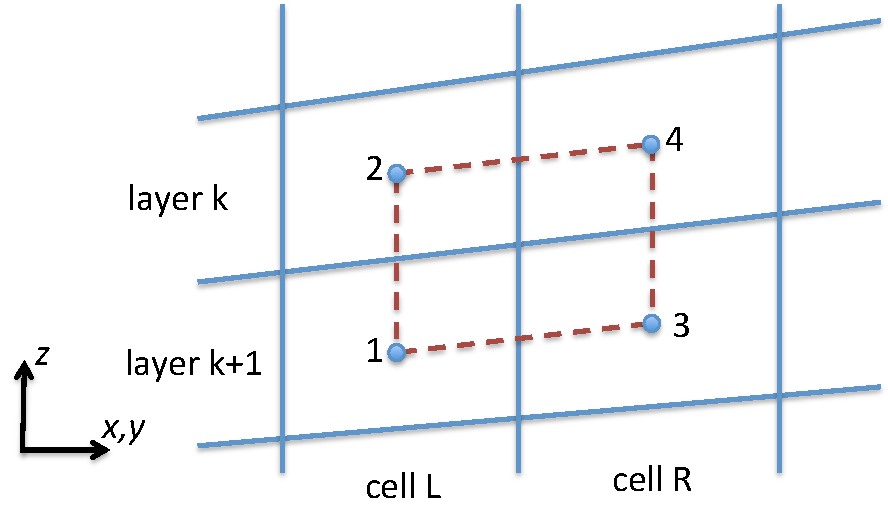
\includegraphics[width=3.5in]{ocean/figures/common_level.pdf}
\caption{Vertical cross-section of ocean grid cells, showing index locations for common level method.  The dots are placed at cell centers in the horizontal and layer mid-depth in the vertical.}
\label{oceanFigure:common level}
\end{figure}

{\bf \large config\_pressure\_gradient\_type = 'Jacobian\_from\_density'}\\
In this formulation the pressure gradient is rewritten in terms of a sea surface height gradient and the vertical integral of a Jacobian,
\begin{eqnarray}
\label{ocean:grad p Jacobian}
- \frac{1}{\rho_0}\nabla_z p &=& - \frac{\rho_s g}{\rho_0}\nabla_s \zeta - \frac{g}{\rho_0}\int_z^\zeta {\mathcal J}(\rho,z)ds, \\
{\mathcal J}(\rho,z) &=& \left. \frac{\partial \rho}{\partial x} \right|_s \frac{\partial z}{\partial s} 
 - \frac{\partial \rho}{\partial s}  \left. \frac{\partial z}{\partial x} \right|_s 
\end{eqnarray}
where $x$ is a general horizontal direction between two cell centers and $s$ is the vertical coordinate reference, i.e.\ $s$ is constant within a layer.  There are many methods to discretize the Jacobian term.  In the common level method, the density is linearly interpolated or extrapolated within each vertical column to a common level $z_\gamma$ (see Figure \ref{oceanFigure:common level}):
\begin{eqnarray}
- \int_z^\zeta {\mathcal J}(\rho,z)ds &=& \overline{\Delta z} \left( \rho^L - \rho^R \right) \\
\overline{\Delta z} &=& \frac{1}{2} \left(z_2-z_1 + z_4-z_3\right) \\
\rho^L &=& \frac{\rho_1\left(z_2-z_\gamma\right) + \rho_2\left(z_\gamma-z_1\right) }{z_2-z_1}\\
\rho^R &=& \frac{\rho_3\left(z_4-z_\gamma\right) + \rho_4\left(z_\gamma-z_3\right) }{z_4-z_3}\\
z_\gamma &=& \left(1-\gamma\right)z_* + \gamma z_c \\
z_* &=&  \frac{z_4 z_2-z_3z_1}{z_4-z_3 + z_2-z_1} \\
z_c &=&  \frac{z_1+z_2+z_3+z_4}{4} 
\end{eqnarray}
where $z_c$ is the depth for the weighted Jacobian method by \citet{Song98mwr}, and $z_*$ is the depth for the standard Jacobian method, which is the depth of intersection of the diagonals of the trapezoidal element in Figure \ref{oceanFigure:common level}.  Here $\gamma$ weights the choice between these two methods for computing the common level $z_\gamma$.  This formulation for the pressure gradient is described in detail in \citet{Shchepetkin_McWilliams03jgr}, Section 2, method 2, and Section 4.  They found that a coefficient of $\gamma=0.5$, which gives equal weights to the standard and weighted Jacobian methods, minimizes the errors in a seamount test problem.

{\bf \large config\_pressure\_gradient\_type = 'Jacobian\_from\_TS'}\\
This formulation is the same as the previous, except that the Jacobian is computed using a linear expansion in potential temperature and salinity.  This option must be used when layers are extremely tilted, such as with sigma coordinates or under an ice shelf, in combination with a nonlinear equation of state.
\begin{eqnarray}
 {\mathcal J}(\rho,z) &=& -\alpha  {\mathcal J}(\theta,z) + \beta  {\mathcal J}(S,z), 
\end{eqnarray}
where
\begin{eqnarray}
\alpha\left( \theta, S, p\right) &=&  -\left. \frac{\partial \rho}{\partial \theta} \right|_{S,p} \\
\beta\left( \theta, S, p\right) &=&  \left. \frac{\partial \rho}{\partial S} \right|_{\theta,p} 
\end{eqnarray}
are the thermal expansion and saline contraction coefficients, computed at a particular  $\left(\theta, S, p\right)$ by the equation of state \citep[eqn 7.16]{Shchepetkin_McWilliams03jgr}.

{\bf \large config\_pressure\_gradient\_type = 'MontgomeryPotential'}\\
For isopycnal vertical coordinates, the user may choose to use the Montgomery potential,
\begin{equation}
\label{ocean:Montgomery Potential}
M = \frac{1}{\rho}p+gz
\end{equation}
and replace the pressure terms above with
\begin{equation}
- \nabla_s M.
\end{equation}
See \citet[section 2.1]{Higdon05jcp} for details on the derivation and computation of the Montgomery potential.

% {\bf \large config\_pressure\_gradient\_type = 'MontgomeryPotential\_and\_density'}
% Same as previous, but this formulation includes an extra term,
% \begin{equation}
% - \nabla_s M + p \nabla_s\left(\frac{1}{\rho} \right),
% \end{equation}
% as described by \citet{Bleck02om}, eqn 1 and end of Appendix A.  This formulation has not been extensively tested and is not supported at this time.

\vspace{0.5in}
{\small
\begin{center}
\begin{longtable}{| p{2.0in} || p{4.0in} |}
	\hline
	{\bf Name} & {\bf Description} \endfirsthead
	\hline 
	{\bf Name} & {\bf Description} (Continued) \endhead
	\hline
	\hline
	\hyperref[subsec:nm_sec_config_pressure_gradient_type]{config\_pressure\_gradient\_type} & Form of pressure gradient terms in momentum equation. For most applications, the gradient of pressure and layer mid-depth are appropriate.  For isopycnal coordinates, one may use the gradient of the Montgomery potential. \\
	\hline
	\hyperref[subsec:nm_sec_config_density0]{config\_density0} &  Density used as a coefficient of the pressure gradient terms,  $\rho_0$ .  This is a constant due to the Boussinesq approximation. \\
	\hline
	\hyperref[subsec:nm_sec_config_common_level_weight]{config\_common\_level\_weight} &  The weight between standard Jacobian and weighted Jacobian,  $\gamma$ . \\
	\hline
\end{longtable}
\end{center}
}
\section[eos]{\hyperref[sec:nm_sec_eos]{eos}}
\label{sec:nm_tab_eos}
Two forms of EOS are supported. The full EOS from \cite{Jackett_McDougall95jaot} and a linear EOS.

\vspace{0.5in}
{\small
\begin{center}
\begin{longtable}{| p{2.0in} || p{4.0in} |}
	\hline
	{\bf Name} & {\bf Description} \endfirsthead
	\hline 
	{\bf Name} & {\bf Description} (Continued) \endhead
	\hline
	\hline
	\hyperref[subsec:nm_sec_config_eos_type]{config\_eos\_type} & Character string to choose EOS formulation \\
	\hline
\end{longtable}
\end{center}
}
\section[eos\_linear]{\hyperref[sec:nm_sec_eos_linear]{eos\_linear}}
\label{sec:nm_tab_eos_linear}
The linear equation of state (leos) is specified as follows:
\begin{equation}
\rho = \rho_{ref} - \alpha_{leos}(T-T_{ref})+\beta_{leos}(S-S_{ref})
\end{equation}
\vspace{0.5in}
{\small
\begin{center}
\begin{longtable}{| p{2.0in} || p{4.0in} |}
	\hline
	{\bf Name} & {\bf Description} \endfirsthead
	\hline 
	{\bf Name} & {\bf Description} (Continued) \endhead
	\hline
	\hline
	\hyperref[subsec:nm_sec_config_eos_linear_alpha]{config\_eos\_linear\_alpha} & Linear thermal expansion coefficient \\
	\hline
	\hyperref[subsec:nm_sec_config_eos_linear_beta]{config\_eos\_linear\_beta} & Linear haline contraction coefficient \\
	\hline
	\hyperref[subsec:nm_sec_config_eos_linear_Tref]{config\_eos\_linear\_Tref} & Reference temperature \\
	\hline
	\hyperref[subsec:nm_sec_config_eos_linear_Sref]{config\_eos\_linear\_Sref} & Reference salinity \\
	\hline
	\hyperref[subsec:nm_sec_config_eos_linear_densityref]{config\_eos\_linear\_densityref} & Reference density, i.e. density when T=Tref and S=Sref \\
	\hline
\end{longtable}
\end{center}
}
\section[split\_explicit\_ts]{\hyperref[sec:nm_sec_split_explicit_ts]{split\_explicit\_ts}}
\label{sec:nm_tab_split_explicit_ts}
The split explicit time-stepping method solves the barotropic (vertically-integrated) velocities separately from the remaining baroclinic velocities.  The time step for the barotropic solve is limited by fast surface gravity waves, and so is subcycled within a large timestep of the baroclinic velocity solve.  This provides a 10 to 12-times speed-up over fourth-order Runge-Kutta time stepping.

A single large timestep in the split explicit algorithm may be summarized as
\begin{itemize}
\item Stage 1: solve for baroclinic velocity (3D)
\item Stage 2: solve for barotropic velocity (2D) with explicit sub-cycling
\item Stage 3: update thickness, tracers, density and pressure
\end{itemize}
The algorithm includes iterations within stage 1, within each subcycle of stage 2, and over the full three-stage process.  Further details are provided in \citet[Appendix A.5]{Ringler_ea13om}

\vspace{0.5in}
{\small
\begin{center}
\begin{longtable}{| p{2.0in} || p{4.0in} |}
	\hline
	{\bf Name} & {\bf Description} \endfirsthead
	\hline 
	{\bf Name} & {\bf Description} (Continued) \endhead
	\hline
	\hline
	\hyperref[subsec:nm_sec_config_n_ts_iter]{config\_n\_ts\_iter} & number of large iterations over stages 1-3 \\
	\hline
	\hyperref[subsec:nm_sec_config_n_bcl_iter_beg]{config\_n\_bcl\_iter\_beg} & number of iterations of stage 1 (baroclinic solve) on the first split-explicit iteration \\
	\hline
	\hyperref[subsec:nm_sec_config_n_bcl_iter_mid]{config\_n\_bcl\_iter\_mid} & number of iterations of stage 1 (baroclinic solve) on any split-explicit iterations between first and last \\
	\hline
	\hyperref[subsec:nm_sec_config_n_bcl_iter_end]{config\_n\_bcl\_iter\_end} & number of iterations of stage 1 (baroclinic solve) on the last split-explicit iteration \\
	\hline
	\hyperref[subsec:nm_sec_config_n_btr_subcycles]{config\_n\_btr\_subcycles} & number of barotropic subcycles in stage 2 \\
	\hline
	\hyperref[subsec:nm_sec_config_n_btr_cor_iter]{config\_n\_btr\_cor\_iter} & number of iterations of the velocity corrector step in stage 2 \\
	\hline
	\hyperref[subsec:nm_sec_config_vel_correction]{config\_vel\_correction} & If true, the velocity correction term is included in the horizontal advection of thickness and tracers \\
	\hline
	\hyperref[subsec:nm_sec_config_btr_subcycle_loop_factor]{config\_btr\_subcycle\_loop\_facto-}\hyperref[subsec:nm_sec_config_btr_subcycle_loop_factor]{r}&  Barotropic subcycles proceed from  $t$  to  $t+n\Delta t$ , where  $n$  is this configuration option. \\
	\hline
	\hyperref[subsec:nm_sec_config_btr_gam1_velWt1]{config\_btr\_gam1\_velWt1} & Weighting of velocity in the SSH predictor step in stage 2.  When zero, previous subcycle time is used; when one, new subcycle time is used. \\
	\hline
	\hyperref[subsec:nm_sec_config_btr_gam2_SSHWt1]{config\_btr\_gam2\_SSHWt1} & Weighting of SSH in the velocity corrector step in stage 2.  When zero, previous subcycle time is used; when one, new subcycle time is used. \\
	\hline
	\hyperref[subsec:nm_sec_config_btr_gam3_velWt2]{config\_btr\_gam3\_velWt2} & Weighting of velocity in the SSH corrector step in stage 2.  When zero, previous subcycle time is used; when one, new subcycle time is used. \\
	\hline
	\hyperref[subsec:nm_sec_config_btr_solve_SSH2]{config\_btr\_solve\_SSH2} & If true, execute the SSH corrector step in stage 2 \\
	\hline
\end{longtable}
\end{center}
}
\section[testing]{\hyperref[sec:nm_sec_testing]{testing}}
\label{sec:nm_tab_testing}
\section{Testing}
\label{sec:testing}

\vspace{0.5in}
{\small
\begin{center}
\begin{longtable}{| p{2.0in} || p{4.0in} |}
	\hline
	{\bf Name} & {\bf Description} \endfirsthead
	\hline 
	{\bf Name} & {\bf Description} (Continued) \endhead
	\hline
	\hline
	\hyperref[subsec:nm_sec_config_conduct_tests]{config\_conduct\_tests} & If true, run testing suite.  This is the overarching control on the test suite.  Individual flags must be set to true below to conduct each test. \\
	\hline
	\hyperref[subsec:nm_sec_config_test_tensors]{config\_test\_tensors} & If true, tensor operations are tested upon start-up. \\
	\hline
	\hyperref[subsec:nm_sec_config_tensor_test_function]{config\_tensor\_test\_function} & Character string to choose tensor test fuction \\
	\hline
\end{longtable}
\end{center}
}
\section[debug]{\hyperref[sec:nm_sec_debug]{debug}}
\label{sec:nm_tab_debug}
At run-time a user can enable debugging features within MPAS-Ocean. These
features include disabling any tendencies to help determine why an issue might
be happening. Debugging options also include various checks on certain fields,
and the ability to prescribe both a thickness and velocity field at run-time
which are constant throughout a simulation. All options that control these
debugging features are specified within the debug namelist record.

\vspace{0.5in}
{\small
\begin{center}
\begin{longtable}{| p{2.0in} || p{4.0in} |}
	\hline
	{\bf Name} & {\bf Description} \endfirsthead
	\hline 
	{\bf Name} & {\bf Description} (Continued) \endhead
	\hline
	\hline
	\hyperref[subsec:nm_sec_config_check_zlevel_consistency]{config\_check\_zlevel\_consistency} & Enables a run-time check for consistency for a zlevel grid. Ensures relevant variables correctly define the bottom of the ocean. \\
	\hline
	\hyperref[subsec:nm_sec_config_filter_btr_mode]{config\_filter\_btr\_mode} & Enables filtering of the barotropic mode. \\
	\hline
	\hyperref[subsec:nm_sec_config_prescribe_velocity]{config\_prescribe\_velocity} & Enables a prescribed velocity field. This velocity field is read on input, and remains constant through a simulation. \\
	\hline
	\hyperref[subsec:nm_sec_config_prescribe_thickness]{config\_prescribe\_thickness} & Enables a prescribed thickness field. This thickness field is read on input, and remains constant through a simulation. \\
	\hline
	\hyperref[subsec:nm_sec_config_include_KE_vertex]{config\_include\_KE\_vertex} & If true, the kinetic energy in each cell is computed by blending cell-based and vertex-based values of kinetic energy. \\
	\hline
	\hyperref[subsec:nm_sec_config_check_tracer_monotonicity]{config\_check\_tracer\_monotonici-}\hyperref[subsec:nm_sec_config_check_tracer_monotonicity]{ty}& Enables a change on tracer monotonicity at the end of the monotonic advection routine. Only used if config\_monotonic is set to .true. \\
	\hline
	\hyperref[subsec:nm_sec_config_disable_thick_all_tend]{config\_disable\_thick\_all\_tend} & Disables all tendencies on the thickness field. \\
	\hline
	\hyperref[subsec:nm_sec_config_disable_thick_hadv]{config\_disable\_thick\_hadv} & Disable tendencies on the thickness field from horizontal advection. \\
	\hline
	\hyperref[subsec:nm_sec_config_disable_thick_vadv]{config\_disable\_thick\_vadv} & Disables tendencies on the thickness field from vertical advection. \\
	\hline
	\hyperref[subsec:nm_sec_config_disable_thick_sflux]{config\_disable\_thick\_sflux} & Disables tendencies on the thickness field from surface fluxes. \\
	\hline
	\hyperref[subsec:nm_sec_config_disable_vel_all_tend]{config\_disable\_vel\_all\_tend} & Disables all tendencies on the velocity field. \\
	\hline
	\hyperref[subsec:nm_sec_config_disable_vel_coriolis]{config\_disable\_vel\_coriolis} & Diables tendencies on the velocity field from the Coriolis force. \\
	\hline
	\hyperref[subsec:nm_sec_config_disable_vel_pgrad]{config\_disable\_vel\_pgrad} & Disables tendencies on the velocity field from the horizontal pressure gradient. \\
	\hline
	\hyperref[subsec:nm_sec_config_disable_vel_hmix]{config\_disable\_vel\_hmix} & Disables tendencies on the velocity field from horizontal mixing. \\
	\hline
	\hyperref[subsec:nm_sec_config_disable_vel_windstress]{config\_disable\_vel\_windstress} & Disables tendencies on the velocity field from horizontal wind stress. \\
	\hline
	\hyperref[subsec:nm_sec_config_disable_vel_vmix]{config\_disable\_vel\_vmix} & Disables tendencies on the velocity field from vertical mixing. \\
	\hline
	\hyperref[subsec:nm_sec_config_disable_vel_vadv]{config\_disable\_vel\_vadv} & Disables tendencies on the velocity field from vertical advection. \\
	\hline
	\hyperref[subsec:nm_sec_config_disable_tr_all_tend]{config\_disable\_tr\_all\_tend} & Disables all tendencies on tracer fields. \\
	\hline
	\hyperref[subsec:nm_sec_config_disable_tr_adv]{config\_disable\_tr\_adv} & Disables tendencies on tracer fields from advection, both horizontal and vertical. \\
	\hline
	\hyperref[subsec:nm_sec_config_disable_tr_hmix]{config\_disable\_tr\_hmix} & Disables tendencies on tracer fields from horizontal mixing. \\
	\hline
	\hyperref[subsec:nm_sec_config_disable_tr_vmix]{config\_disable\_tr\_vmix} & Disables tendencies on tracer fields from vertical mixing. \\
	\hline
	\hyperref[subsec:nm_sec_config_disable_tr_sflux]{config\_disable\_tr\_sflux} & Disables tendencies on tracer fields from surface fluxes. \\
	\hline
\end{longtable}
\end{center}
}
